% !TEX root =../thesis-letomes.tex

\chapter{Results}
The main aim of the project was twofold: to examine whether or not ES was a reasonable method to apply in this problem space, and to create a mars mission simulator to compare it with the lunar case, under the expectation that the two problems would be more or less similar. We have accomplished both these things, certainly, even though they did not take the shape we were initially expecting. In this chapter we will examine the various threads in the knotted mess that is this project, to see where they ended up.

\section{Evolution Strategies' fitness for this problem space}
We implemented several versions of the fundamental ES concept, with different combinations of additions that have given good results in the literature. Certain additions had more impact than others, but no matter what variation we used, the results weren't exactly earth-shattering. The problem space has a fractured, fractal quality of very good solutions hiding among very bad ones. These solutions are not found in any particularly ingenious fashion by ES, nor by any gradiend descent method, really. There are areas of good structure, where ES finds a local minimum just fine, but if the objective is simply to find a decent solution, then something naive like random guessing will also perform well, since the space is sufficiently dense with decent solutions. 

When we computed the problem space flattened to two dimensions by locking the burn-angle to 0, we gained valuable information and intuition about its shape. 

\begin{figure}[h]
    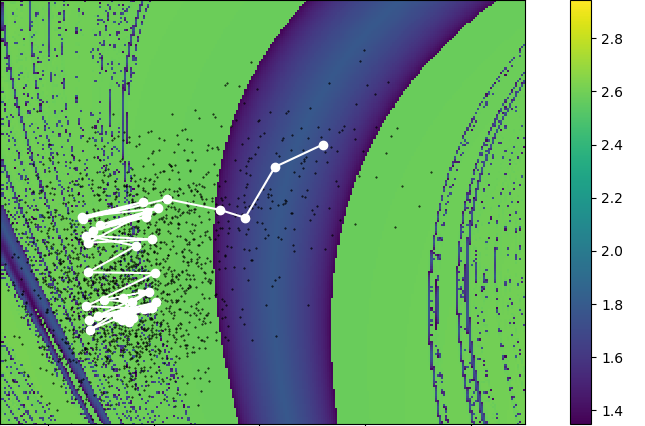
\includegraphics{fig/inESdivergingfromridge.png}
    \caption{Here we see the fractured, unorganized region pulling us away from the ridge}
    \label{fig:esdivergingfromridge}
\end{figure}



\section{Finding LETOs to Mars}

